\scanpage{29}
\deleted{$\unsure{(i+p-1)p-(i+p-2)p}$}
\diagram{\begin{tikzcd}E\arrow[r,"u"]&F\\\omega&\omega'\end{tikzcd}}
\[\boxed{u\circ\omega=du+\omega'\circ u}\]
\[
(i+p)(p+1)-(i+p-1)p=\deleted{ip}+\deleted{p^2}+i+p-\deleted{ip}-\deleted{p^2}+p=\uline{2p+i}
\]
\deleted{$\unsure{E_{0S}}\longrightarrow E_S$}
\figure{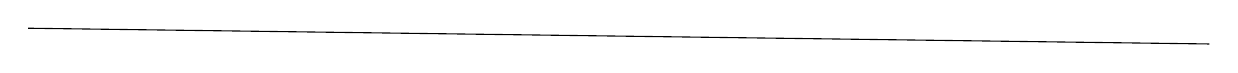
\begin{tikzpicture}\draw (0,.2)--(15,0);\end{tikzpicture}}
\deleted{$\unsure{E_{0S}}$}\quad\deleted{$\unsure{\varphi}$}
\diagram{\begin{tikzcd}[column sep=small,row sep=small]
S_0\arrow[r,dash]\arrow[d,dash]&S\arrow[d,dash]\\
k\arrow[r,dash]&W
\end{tikzcd}}
$F_S\qquad\deleted{F_S^*}\lambda\qquad\deleted{\unsure{\sigma_{E_S}}}$
\diagram{\begin{tikzcd}[column sep=small,row sep=small]
S\arrow[rr,dash,bend left,"F_S"]\arrow[d,dash]&&S\arrow[d,dash]\\
\operatorname{Spec}(W)\arrow[rr,"F_W"]\arrow[dr,dash]&&\operatorname{Spec}(W)\arrow[dl,dash]\\
&\operatorname{Spec}\mathbb Z_p&
\end{tikzcd}}
\[M=E_W\qquad E\text{ module libre de t.f.}\]
\[\deleted{F_S^*(E_W)=E_W^\sigma}\qquad\unsure{E^{\sigma'}}\]
\diagram{\begin{tikzcd}[column sep=small,row sep=small]
F_S^*(E_S)\arrow[r,"F_M"]&E_S\\
E_S\arrow[u,phantom,"\wr"]\arrow[ur,"\Phi"']&
\end{tikzcd}}
$\Phi$ \uuline{induit un isom} après $\otimes_{\mathbb Z_p}\mathbb Q_p$
\[
\unsure{A}\in\Gamma(\widehat\Omega^1_{S/W}\otimes\operatorname{End}(E_S))
\]
\[
\unsure{A'}=F_S^*(\nabla)\in\Gamma\left(\widehat\Omega^1_{S/W}\otimes\underbrace{\operatorname{End}(F_S^*(E_S))}_{\wr\ \operatorname{End}(E_S)}\right)
\]
\deleted{$\unsure{\Phi}$}\qquad\deleted{$\Phi\circ\nabla$}
\[
\Phi\circ A^\sigma=d\Phi+A\circ\Phi
\]
i.e.
\[\boxed{d\Phi=\Phi\circ A^\sigma-A\circ\Phi}\]
\margin{exprime que $F_M$ est compatible à la connexion}
\deleted{$K(A)=$}
\[\boxed{dA+[A,A]=0}\]
\margin{exprime que \inserted{la connexion} $\nabla$ définie par $A$ est à courbure nulle}
\deleted{$\Phi^{-1}$}
\[
\exists\Psi:E_S\mathbin{-}E_S,\quad\text{et }i,\text{ tel que}
\]
\[\boxed{\Psi\Phi=p^i\mathrm{id}}\]
\mspage{28}
